\documentclass{beamer}

\mode<presentation> {
  \usepackage{comment}
  \usepackage{pgfgantt}
  \usetheme{Madrid}
}

\usepackage{graphicx} 
\usepackage{booktabs} 
\usepackage{enumerate}
\usepackage{ragged2e}

%======================================================================================================
%======================================================================================================

\title[NVAT]{Novel Video Analytics and Tapestry}
\logo{
\includegraphics[width=.8cm,keepaspectratio]{logo.png}}

\author[]{
  V. Alekhya
\newline
  Nadimpalli Vineetha
\newline
  Tarun Rajnish
\newline	
  Mohammed Talha Zubair
\newline
\newline
\small{
  Dr.Suryaprasad J
\newline  Batch No. 25}}

\institute[25]{}

\date[November 8, 2017]{November 8, 2017} 

%------------------------------------------------------------------------------------------------------

\begin{document}

%------------------------------------------------------------------------------------------------------
% SLIDE 1

\begin{frame}
  \titlepage 
\end{frame}

%------------------------------------------------------------------------------------------------------
% SLIDE 2

\section{Motivation}
\begin{frame}{Motivation of the Work}
  \textit{\large{Then}}
  \begin{itemize}
    \item Humans did bulk of the work
    \item Accessed hours of video data
    \item Tedious and cumbersome
    \item Human error or oversight
  \end{itemize} 
  \begin{center}
    \textbf{\textcolor{blue}{\Large{Need to eliminate human intervention}}}
  \end{center}
  \textit{\large{Now}}
  \begin{itemize}
    \item VMD system monitors all cameras in the network
    \item Reacts only when there is suspicious activity
  \end{itemize}    	
\end{frame}

%------------------------------------------------------------------------------------------------------
% SLIDE 3

\section{Problem Statement}
\begin{frame}{Problem Statement}
  \begin{itemize}
    \item Video content analysis - analyze video to detect and determine temporal and spatial events
    \item Purpose of ensuring safety and security
  \end{itemize}
  Our Attempt:
  \begin{itemize}
    \item Detect unwanted access (intruders)
    \item Process the data obtained from CCTV footage via various video stitching techniques 
  \end{itemize}
\end{frame}

%------------------------------------------------------------------------------------------------------
% SLIDE 4

\section{VAT}
\begin{frame}{VAT \\ (Video Analytics and Tapestry)}
  We would focus on the feature of producing a
  \begin{center}
    \textbf{\textcolor{blue}{\Large{time line depicting the path travelled}}}
  \end{center}
  by the intruder, computed from the feed of multiple cameras in the network
\end{frame}

%------------------------------------------------------------------------------------------------------
% SLIDE 5

\section{Block diagram}
\begin{frame}{High level block diagram}
  \begin{center}
    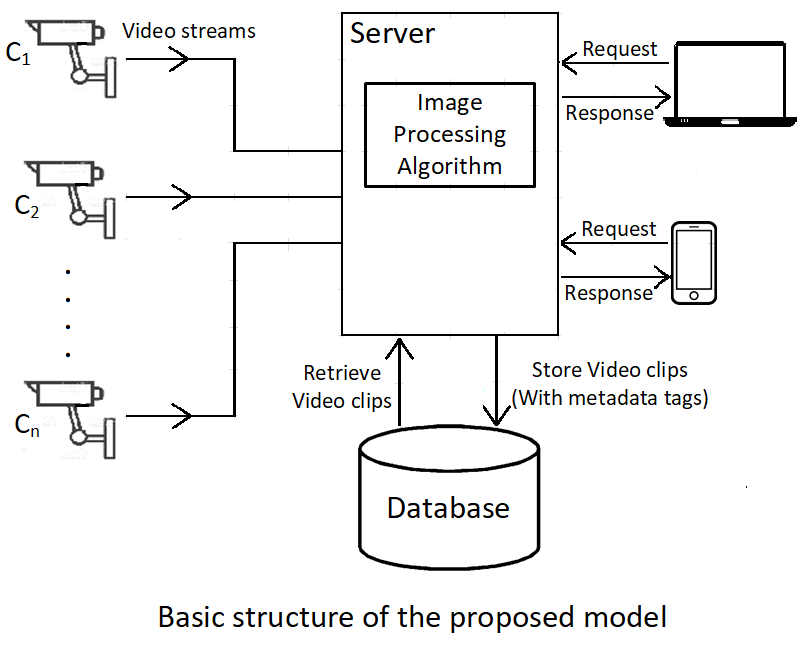
\includegraphics[width=10cm,keepaspectratio]{HighLevelBlockDiagram.png}
  \end{center}
\end{frame}

%------------------------------------------------------------------------------------------------------
% SLIDE 6

\section{Methodology}
\begin{frame}{Proposed methodology}
\begin{enumerate}[1.]
\item Video clips from cameras on the network 
\item Image/Video processing algorithms
	  \begin{itemize}
	  \item Add metadata to each clip
      	\begin{itemize}
      	\item Camera ID
      	\item Timestamp
      	\item .....
      	\end{itemize}
	  \item Store video clips
      \item Check for intruder
        \begin{itemize}[ ]
        \item (if detected)
        \item -Retrieve video clips of neighbouring cameras
        \item (repeat)
        \item -link video clips(tapestry)
        \end{itemize}
	  \end{itemize}
\item Analytics and statistics
\end{enumerate}
\end{frame}

%------------------------------------------------------------------------------------------------------
% SLIDE 7

\section{Literature Survey} 
\begin{frame}{Literature Survey}
  \begin{itemize}
    %\justifying
    \item Andrew A. Adams and James M. Ferryman discuss the three stages of a surveillance system. The first stage of people and/or object monitoring is detection and classification which consists of localizing new objects entering the surveillance area.
    \newline
    \item White Paper Agent Video Intelligence introduces an architectural approach to Video Analytics. With Agent VI’s architecture, the Video Analytics task is distributed between the edge device (which may be an IP camera or encoder) and a server.
   
  \end{itemize}
\end{frame}

%------------------------------------------------------------------------------------------------------
% SLIDE 8
\section{Literature Survey} 
\begin{frame}{Literature Survey}
  \begin{itemize}
    %\justifying
   
    \item Frost \& Sullivan mention in their white paper that the core of IBM's Intelligent Video Analytics solution deals with the application of analytic and information management tools to the available video data. It can process the video data in real time to extract events (activities in the camera’s field of view) and classify the events or objects in them in multiple ways, including generating metadata on them.
  \end{itemize}
\end{frame}

%------------------------------------------------------------------------------------------------------
% SLIDE 9
\section{Schedule}
\begin{frame}
\frametitle{Time line of completion of project from Nov 2017-10th April 2018(Gantt Charts).}
\definecolor{barblue}{RGB}{153,204,254}
\definecolor{groupblue}{RGB}{51,102,254}
\definecolor{linkred}{RGB}{165,0,33}
\renewcommand\sfdefault{phv}
\renewcommand\mddefault{mc}
\renewcommand\bfdefault{bc}
\setganttlinklabel{s-s}{START-TO-START}
\setganttlinklabel{f-s}{FINISH-TO-START}
\setganttlinklabel{f-f}{FINISH-TO-FINISH}
\sffamily
\begin{ganttchart}[
    canvas/.append style={fill=none, draw=black!5, line width=.75pt},
    hgrid style/.style={draw=black!5, line width=.75pt},
    vgrid={*1{draw=black!5, line width=.75pt}},
    today=7,
    today rule/.style={
      draw=black!64,
      dash pattern=on 3.5pt off 4.5pt,
      line width=1.5pt
    },
    today label font=\small\bfseries,
    title/.style={draw=none, fill=none},
    title label font=\bfseries\footnotesize,
    title label node/.append style={below=7pt},
    include title in canvas=false,
    bar label font=\mdseries\small\color{black!70},
    bar label node/.append style={left=2cm},
    bar/.append style={draw=none, fill=black!63},
    bar incomplete/.append style={fill=barblue},
    bar progress label font=\mdseries\footnotesize\color{black!70},
    group incomplete/.append style={fill=groupblue},
    group left shift=0,
    group right shift=0,
    group height=.5,
    group peaks tip position=0,
    group label node/.append style={left=.6cm},
    group progress label font=\bfseries\small,
    link/.style={-latex, line width=1.5pt, linkred},
    link label font=\scriptsize\bfseries,
    link label node/.append style={below left=-2pt and 0pt}
  ]{1}{13}
  \gantttitle[
    title label node/.append style={below left=7pt and -3pt}
  ]{WEEKS:\quad1}{1}
  \gantttitlelist{2,...,13}{1} \\
  \ganttgroup[progress=20]{Summary Element 1}{1}{10} \\
  \ganttbar[
    progress=80,
    name=WBS1A
  ]{\textbf{1} Problem Statement and Survey}{1}{3} \\
  \ganttbar[
    progress=0,
    name=WBS1B
  ]{\textbf{2} System Requirement Specification}{3}{5} \\
  \ganttbar[
    progress=0,
    name=WBS1C
  ]{\textbf{3} Defining Intrusion and Tapestry}{5}{11} \\
  \ganttbar[
    progress=0,
    name=WBS1D
  ]{\textbf{4} GUI, Analytics and Final Testing}{11}{15} \\[grid]
  
\end{ganttchart}

%\begin{columns}[c] % The "c" option specifies centered vertical alignment while the "t" option is used for top vertical alignment

%\column{.45\textwidth} % Left column and width
%\textbf{Heading}
%\begin{enumerate}
%\item Statement
%\item Explanation
%\item Example
%\end{enumerate}

%\column{.5\textwidth} % Right column and width
%Lorem ipsum dolor sit amet, consectetur adipiscing elit. Integer lectus nisl, ultricies in feugiat rutrum, porttitor sit amet augue. Aliquam ut tortor mauris. Sed volutpat ante purus, quis accumsan dolor.

%\end{columns}
\end{frame}

%------------------------------------------------------------------------------------------------------
% SLIDE 10

\section{Schedule}
\begin{frame}{Gantt chart}
  \begin{center}
    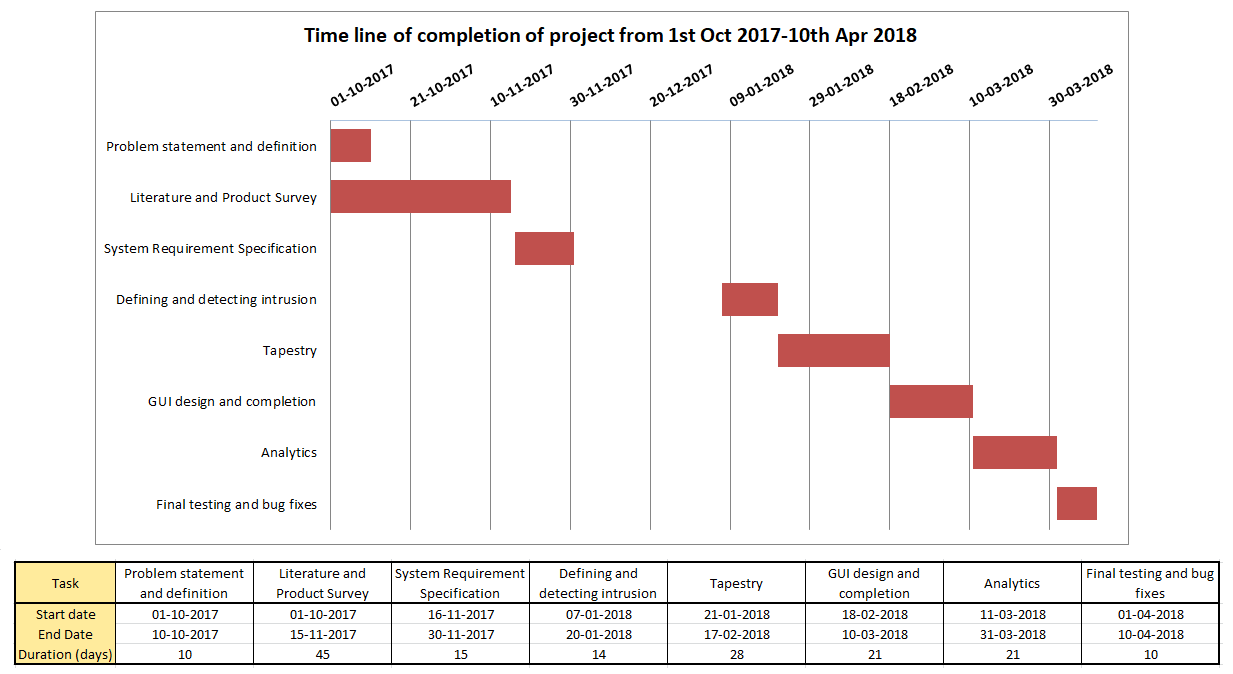
\includegraphics[width=12cm,keepaspectratio]{GanttChart.png}
  \end{center}
\end{frame}

%------------------------------------------------------------------------------------------------------
% SLIDE 11

\section{Outcome}
\begin{frame}{Proposed Outcome}
\begin{block}{1.}
Tapestry of video clips
\end{block}

\begin{block}{2.}
Detection of intruder(Non-staff, non-student,...)
\end{block}

\begin{block}{3.}
Analytics on surveillance data
\end{block}

\begin{block}{4.}
Open source datasets
\end{block}
\end{frame}

%------------------------------------------------------------------------------------------------------
% SLIDE 12

\section{References}
\begin{frame}{References}
  \footnotesize{
  \begin{thebibliography}{99}
    \bibitem{p1} James  M. Ferryman, Andrew A. Adams
    \newblock The future of video analytics for surveillance and its ethical implications
    \newblock \emph{Security Journal, 2012}

    \bibitem{p1} AGENT VI
    \newblock White paper agent video intelligence tech. rep.,
    \newblock \emph{JULY 2016}

    \bibitem{p1} B. Cotton
    \newblock Enhancing a city’s ability to plan, protect and manage with intelligent video analytics, 				  Tech. Rep. 
    \newblock GPW12348-USEN-00 
    \newblock \emph{A Frost \& Sullivan White paper}
  \end{thebibliography}
  }
\end{frame}

%------------------------------------------------------------------------------------------------------
% SLIDE 13

\begin{frame}
\textcolor{blue}{\Huge{\centerline{The End}}}
\end{frame}

%------------------------------------------------------------------------------------------------------

\end{document}

%======================================================================================================
%======================================================================================================
